\documentclass[letterpaper]{article} % DO NOT CHANGE THIS
\usepackage[submission]{aaai2027}  % DO NOT CHANGE THIS
% The serif, sans-serif, and monospaced fonts are loaded automatically by
% aaai2027.sty (newtxtext, helvet, courier). DO NOT add \usepackage{times},
% \usepackage{helvet}, \usepackage{courier}, or any other font package.
\usepackage[hyphens]{url}  % DO NOT CHANGE THIS
\usepackage{graphicx} % DO NOT CHANGE THIS
\urlstyle{rm} % DO NOT CHANGE THIS
\def\UrlFont{\rm}  % DO NOT CHANGE THIS
\usepackage{natbib}  % DO NOT CHANGE THIS AND DO NOT ADD ANY OPTIONS TO IT
\usepackage{caption} % DO NOT CHANGE THIS AND DO NOT ADD ANY OPTIONS TO IT
\frenchspacing  % DO NOT CHANGE THIS
%
% These are recommended to typeset algorithms but not required. See the subsubsection on algorithms. Remove them if you don't have algorithms in your paper.
\usepackage{algorithm}
\usepackage{algorithmic}

%
% These are recommended to typeset listings but not required. See the subsubsection on listing. Remove this block if you don't have listings in your paper.
\usepackage{newfloat}
\usepackage{listings}
\DeclareCaptionStyle{ruled}{labelfont=normalfont,labelsep=colon,strut=off} % DO NOT CHANGE THIS
\lstset{%
	basicstyle={\footnotesize\ttfamily},% footnotesize acceptable for monospace
	numbers=left,numberstyle=\footnotesize,xleftmargin=2em,% show line numbers, remove this entire line if you don't want the numbers.
	aboveskip=0pt,belowskip=0pt,%
	showstringspaces=false,tabsize=2,breaklines=true}
\floatstyle{ruled}
\newfloat{listing}{tb}{lst}{}
\floatname{listing}{Listing}

%
% Recommended for better-looking tables
\usepackage{booktabs}

%
% Keep the \pdfinfo as shown here. There's no need
% for you to add the /Title and /Author tags.
\pdfinfo{
/TemplateVersion (2027.1)
}

% DISALLOWED PACKAGES
% \usepackage{authblk} -- This package is specifically forbidden
% \usepackage{balance} -- This package is specifically forbidden
% \usepackage{CJK} -- This package is specifically forbidden
% \usepackage{float} -- This package is specifically forbidden
% \usepackage{flushend} -- This package is specifically forbidden
% \usepackage{fullpage} -- This package is specifically forbidden
% \usepackage{geometry} -- This package is specifically forbidden
% \usepackage{hyperref} -- This package is specifically forbidden
% \usepackage{navigator} -- This package is specifically forbidden
% (or any other package that embeds links such as navigator or hyperref)
% \usepackage{indentfirst} -- This package is specifically forbidden
% \usepackage{layout} -- This package is specifically forbidden
% \usepackage{multicol} -- This package is specifically forbidden
% \usepackage{nameref} -- This package is specifically forbidden
% \usepackage{savetrees} -- This package is specifically forbidden
% \usepackage{setspace} -- This package is specifically forbidden
% \usepackage{stfloats} -- This package is specifically forbidden
% \usepackage{tabu} -- This package is specifically forbidden
% \usepackage{titlesec} -- This package is specifically forbidden
% \usepackage{tocbibind} -- This package is specifically forbidden
% \usepackage{ulem} -- This package is specifically forbidden
% \usepackage{wrapfig} -- This package is specifically forbidden
% DISALLOWED COMMANDS
% \nocopyright -- Your paper will not be published if you use this command
% \addtolength -- This command may not be used
% \balance -- This command may not be used
% \baselinestretch -- Your paper will not be published if you use this command
% \clearpage -- No page breaks of any kind may be used for the final version of your paper
% \columnsep -- This command may not be used
% \newpage -- No page breaks of any kind may be used for the final version of your paper
% \pagebreak -- No page breaks of any kind may be used for the final version of your paper
% \pagestyle -- This command may not be used
% \tiny -- This is not an acceptable font size.
% \vspace{- -- No negative value may be used in proximity of a caption, figure, table, section, subsection, subsubsection, or reference
% \vskip{- -- No negative value may be used to alter spacing above or below a caption, figure, table, section, subsection, subsubsection, or reference

\usepackage{xspace}

\setcounter{secnumdepth}{0} %May be changed to 1 or 2 if section numbers are desired.

% The file aaai2027.sty is the style file for AAAI Press
% proceedings, working notes, and technical reports.
%

% ====================  YOUR MACROS (content only, no layout changes)  ====================
\usepackage{amsmath}
\usepackage{amssymb}
\usepackage{amsthm}
\usepackage{xspace}
\usepackage{cleveref}   % \cref / \Cref auto-naming (no hyperref -> no links, AAAI-safe)
\usepackage{tikz}
\newtheorem{theorem}{Theorem}
\newtheorem{lemma}{Lemma}
\newtheorem{definition}{Definition}

% Paper notation -- each name/number changes in one place.
% Names (rename before camera-ready; keep neutral for anonymity):
\newcommand{\methodname}{\textsc{Faithful E}\xspace}   % the methodology (one name)
\newcommand{\dataset}{\textsc{LeanEuclidF}\xspace}    % the released corpus

% Terms kept consistent (not brands):
\newcommand{\mapstage}{mapping stage\xspace}
\newcommand{\fillstage}{completion stage\xspace}

% faithfulness necessary conditions
\newcommand{\faithfulcriteria}{six necessary conditions\xspace}  
\newcommand{\NL}{\ifmmode \text{NL}\else NL\xspace\fi}
\newcommand{\Formal}{\ifmmode \text{Lean}\else Lean\xspace\fi}
\newcommand{\NLtoFormal}[1]{f_{\text{formal}}(#1)}
\newcommand{\NLProof}{P_\text{NL}}

\newcommand{\coverage}{\textsc{Coverage}\xspace}
\newcommand{\totality}{\textsc{Totality}\xspace}
\newcommand{\fidelity}{\textsc{Fidelity}\xspace}
\newcommand{\grounding}{\textsc{Grounding}\xspace}
\newcommand{\constructibility}{\textsc{Constructibility}\xspace}
\newcommand{\locality}{\textsc{Locality}\xspace}

\newcommand{\assert}[1]{\operatorname{assert}(#1)}   % assertion of a sentence
\newcommand{\reason}[1]{\operatorname{reasons}(#1)}   % its reasoning part
\newcommand{\citations}[1]{\operatorname{citations}(#1)}

\newcommand{\numproofs}{99\xspace}

   % notation macros -- edit them in macros.tex (keep it open in a split)
% =========================================================================================

% Title -- mixed case (capitalize verbs/nouns/adjectives; lowercase articles/prepositions)
\title{Faithful Proofs in Euclidian Geometry}

% Anonymous submission: "Anonymous Submission" as sole author, empty affiliations (AAAI rule).
\author{Anonymous Submission}
\affiliations{}

\begin{document}
\maketitle

\begin{abstract}
% TODO abstract (~150--200 words): context, gap, what we do, key result.
\cite{avigad_formal_2009}
\end{abstract}

% Uncomment near submission to link code / data (keep anonymized).
% \begin{links}
%     \link{Code}{https://aaai.org/example/code}
% \end{links}

% =========================================================================================
% PAGE BUDGET (7 pp total). Soft guides -- not enforced.
%   Abstract + Intro ...... 1.5
%   Motivating Example .... 0.75  (+ Figure 0.25)
%   Methodology ........... 1.5   (+ Figure 0.25, + Algorithm 0.25)
%   Evaluation ............ 2.5   (RQ1-RQ5, ~5 figures/tables)
%   Related Work + Concl. . 0.75
% =========================================================================================

\section{Introduction}
% - What problem: faithful formalization of Euclid proofs; gap vs prior (LeanEuclid).
% - Our idea in 2-3 sentences. Contributions as a bulleted list.
Given a natural language (NL) proof, a faithful formalization has many applications; it can be used to check the reasoning of an AI, it can be used to help expert mathematicians verify a large proof, and it is a necessary step to complete textbook level autoformalization. However, the notion of what a faithful proof even is, is not well addressed, nor how we can general faithful proofs. In order to address this, we give a set of \faithfulcriteria a proof must have, that any faithful methodology must ensure, and developped an algorithm \methodname, that guarantees these criteria are satisfied.

The focus of our study was on Euclidian geometry, which is considered formal, so being faithful should not introduce many soundness issues, and an existing system exists \citep{murphy_autoformalizing_2024} and \citep{avigad_formal_2009} helping us get started.

Thus we build off of the Book 1 proofs done by \citet{murphy_autoformalizing_2024}. We address two issues with this work. The first, is that we believe these proofs are not faithful. They do not satisfy our proposed \faithfulcriteria. The second, is that the work of \citet{murphy_autoformalizing_2024} takes very long to compile the formal proof and sometimes may not even compile. \citet{min_divide_2026} had to comment out 10 propositions because of this, and we were unable to compile some of the proofs in under 20 minutes. So we also ensure our methodology generates proofs that compile much faster.

We ran our methodology through Books 1, 2, and 3, generating \numproofs faithful proofs of Euclid's Elements.


\section{Motivating Example}
% One concrete Euclid proposition: show an unfaithful vs faithful proof, motivate the method.

% \begin{figure}[t]
% \centering
% 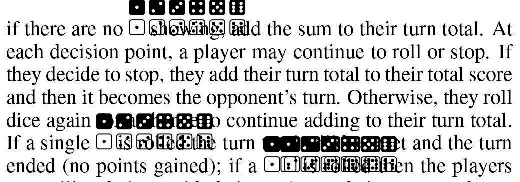
\includegraphics[width=0.9\columnwidth]{Figures/figure1}
% \caption{Motivating example.}
% \label{fig:motivating}
% \end{figure}
\section{Methodology}

Our goal is to generate Lean proofs \emph{guaranteed} to satisfy the \faithfulcriteria and \soundness (\cref{tab:conditions}) with minimal \oracle\footnote{We use human experts, but a capable \llm could serve.} and \llm{} reliance, since the \oracle is the most expensive resource and \llm{} calls cost money. Everything else is a \script: a deterministic procedure that uses no \llm. As \cref{tab:conditions} shows, every condition is checked by a \script or by Lean except \atomicity and \atomicfaithfulness, which the \oracle only \emph{reviews}. \methodname runs in two stages: a \mapstage that translates the NL proof sentence by sentence, and a \fillstage that proves each sentence.


\begin{table*}[t]
\centering
\caption{Conditions our methodology guarantees. An NL proof is a sequence of sentences (substrings of the NL proof), each asserting a mathematical statement, and some with justifying information we refer to as assumptions for this sentence. Script checks are automated with no LLM use, while oracle is checked through human experts.}
\label{tab:conditions}
\begin{tabular}{@{}l p{0.62\textwidth} l@{}}
\toprule
Name & Condition & Checked by \\
\midrule
\multicolumn{3}{@{}l}{\emph{Faithfulness}}\\
\coverage           & The sentences concatenate, in order, to the entire proof & Script \\
\atomicity          & Each sentence makes one assertion with the assumptions it uses (``since $S_1$ and $S_2$, therefore $A$'' has assumptions $S_1, S_2$ and assertion $A$) & Oracle \\
\atomicfaithfulness & Each assertion and assumption is translated to a Lean statement asserting the same thing, in sentence order & Oracle \\
\citcond            & Every proposition Euclid cites is also cited in the Lean proof, in the right place & Script \\
\midrule
\multicolumn{3}{@{}l}{\emph{Soundness}}\\
\soundness          & The Lean proof compiles with no \texttt{sorry} & Lean \\
\bottomrule
\end{tabular}
\end{table*}

\subsection{\mapstage}
The \llm splits the NL proof into sentences it judges atomic (\atomicity). A \script checks \coverage, that the sentences concatenate to the original proof, and the \llm revises until it passes. The \llm then translates each sentence's assertion and assumptions into Lean (\atomicfaithfulness), and a \script \emph{partially} checks \citcond: partially, because citations meant to \emph{prove} a sentence are still \texttt{sorry} at this stage. The \oracle reviews \atomicity and \atomicfaithfulness and returns feedback until satisfied. The result is frozen into a file the \llm cannot edit, the contract the \fillstage must satisfy without weakening it.

\subsection{\fillstage}
Naively, one hands this file, Lean with one \texttt{sorry} per sentence, to the \llm to fill in. For a fully formal NL proof this local gap-filling works. Euclid's is not fully formal: he relies on diagrammatic reasoning, so a sentence like ``therefore $AB=CD$ [Prop.~I.4]'' is rarely one tactic call. Proving it in System E \citep{avigad_formal_2009}, an axiom system for diagram-based Euclidean geometry that Euclid never used, means re-establishing the figure facts he read off the diagram, such as betweenness, side-of-line, and distinctness, as explicit hypotheses for the SMT backend, which again is why Book 1 \citep{murphy_autoformalizing_2024} had long compiling time issues. The backend also may give no signal on failure: \texttt{euclid\_finish} closes a small explicit step but times out on anything larger, with no counterexample and no partial progress, so blind retrying may not converge.

\methodname builds the proof as a rooted DAG (\cref{fig:dag}) and proves it with \cref{alg:prove}. Each \emph{node} is a single Lean lemma, and an \emph{edge} is a \texttt{have} in the parent that invokes a child. The root is the proposition; the \mapstage fixes its sentence-children, \textsc{Prove} discovers the rest, and a shared node is proved once even when several parents use it. Before a node's children are proved, two type-level \script checks gate them: \emph{sufficiency} (SF), that assuming the children's statements lets the node type-check, and \emph{suppliability} (SP), that each child's hypotheses are already present in the parent. To pick an axiom, the \llm queries a \script that indexes the System-E facts by what they conclude and consume.

In Lean a \texttt{sorry} is a term of any type, so a lemma with \texttt{sorry} sub-claims still type-checks; a node therefore compiles without its children, which keeps every compile small and independent. This composes into a sound proof: each leaf is proved outright, each internal node is valid given its children's statements (which SF and SP make it use correctly), and a \script checks that every \texttt{sorry} is discharged by another node, down to the leaves, so the assembled proof has no gaps. Cost is thus bounded by decomposition: splitting deeper shrinks each node's own work until it compiles within a fixed budget, 30 seconds, however large the proof.

\begin{figure}[t]
\centering
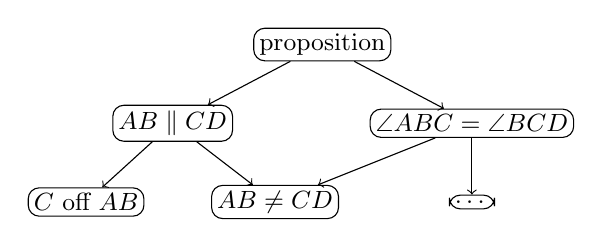
\begin{tikzpicture}[
  nd/.style={draw, rounded corners, inner sep=2pt, font=\small}]
\node[nd] (root) at (0,2) {proposition};
\node[nd] (s1) at (-1.9,1) {$AB \parallel CD$};
\node[nd] (s2) at (1.9,1) {$\angle ABC = \angle BCD$};
\node[nd] (l1) at (-3,0) {$C$ off $AB$};
\node[nd] (l2) at (-0.6,0) {$AB \neq CD$};
\node[nd] (l3) at (1.9,0) {$\dots$};
\draw[->] (root) -- (s1); \draw[->] (root) -- (s2);
\draw[->] (s1) -- (l1);   \draw[->] (s1) -- (l2);
\draw[->] (s2) -- (l2);   \draw[->] (s2) -- (l3);
\end{tikzpicture}
\caption{The proof as a rooted DAG. Each \emph{node} is a claim; an \emph{edge} points to a child it depends on, left \texttt{sorry} while the node is proved so it compiles on its own. The root is the proposition; the leaves depend on nothing. A child shared by two parents ($AB \neq CD$) makes it a DAG rather than a tree.}
\label{fig:dag}
\end{figure}

\begin{algorithm}[t]
\caption{\textsc{Prove}(node $C$): prove $C$, leaving every other node \texttt{sorry}. The whole proof is \textsc{Prove}(root).}
\label{alg:prove}
\begin{algorithmic}[1]
\STATE attempt a direct proof of $C$ and compile it \COMMENT{\llm}
\IF{it compiles}
  \STATE \textbf{return}
\ELSIF{the error is readable}
  \STATE fix it; \textbf{return} \textsc{Prove}($C$) \COMMENT{\llm}
\ENDIF
\REPEAT
  \STATE split $C$ into children $N_1,\dots,N_n$ \COMMENT{\llm}
  \STATE check SF and SP on the children \COMMENT{\script}
\UNTIL{both hold}
\FOR{$i = 1$ to $n$}
  \STATE \textsc{Prove}($N_i$), or re-split $C$ if it was wrong \COMMENT{\llm}
\ENDFOR
\STATE \textbf{return}
\end{algorithmic}
\end{algorithm}

\section{Evaluation}
% ~2.5 columns. Frame around the research questions below.

\subsection{RQ1: Faithfulness of Generated Proofs}
% Our method vs \leaneuclid{}. Human rubric (30+) on Book 1; LLM-as-judge on Books 1--3.
% Report human-judge alignment.

\subsection{RQ2: Synthesis Runtime Under a Finite Budget}
% Our method vs pure LLM-agent baseline, Books 1--3 (not necessarily comprehensive).

\subsection{RQ3: Lean Compile Performance}
% Our artifact vs \leaneuclid{}, Book 1.

\subsection{RQ4: Qualitative Analysis}

\subsection{RQ5: Accept/Refute of LLM-Generated NL Proofs}
% Small scale: apply our methodology to accept/refute an LLM's natural-language proof.

% Example results table:
% \begin{table}[t]
% \centering
% \begin{tabular}{lcc}
% \toprule
% Method & Faithfulness & Runtime \\
% \midrule
% \leaneuclid{} & & \\
% Ours & & \\
% \bottomrule
% \end{tabular}
% \caption{Main results.}
% \label{tab:main}
% \end{table}

\section{Related Work}

\section{Conclusion}

\bibliography{aaai2027}

% Reproducibility checklist -- include only if the conference wants it inline.
% \input{ReproducibilityChecklist.tex}

\end{document}
